% Created 2023-09-16 Sat 16:28
% Intended LaTeX compiler: lualatex
\documentclass[11pt]{article}
\usepackage{graphicx}
\usepackage{longtable}
\usepackage{wrapfig}
\usepackage{rotating}
\usepackage[normalem]{ulem}
\usepackage{amsmath}
\usepackage{amssymb}
\usepackage{capt-of}
\usepackage{hyperref}
\DeclareExerciseCollection{Adaptadas-TeoriaAtomica}
\DeclareExerciseCollection{Adaptadas-Estequiometria}
\DeclareExerciseCollection{Adaptadas-Termoquimica}
\author{fabio}
\date{\today}
\title{}
\hypersetup{
 pdfauthor={fabio},
 pdftitle={},
 pdfkeywords={},
 pdfsubject={},
 pdfcreator={Emacs 28.1 (Org mode 9.5.2)}, 
 pdflang={English}}
\begin{document}

\tableofcontents

\collectexercises{Adaptadas-TeoriaAtomica}

\begin{exercise}
Leia a tirinha abaixo

\begin{center}
\includegraphics[scale=1.5]{Adaptadas/cientistas.pdf}
\end{center}

Qual dos modelos abaixo representa o modelo citado na imagem

\begin{choice}(3)
\choice \includegraphics[scale=.6]{Adaptadas/thomson.jpg}
\choice \includegraphics[scale=.1]{Adaptadas/bilhar.png}
\choice \includegraphics[scale=.2]{Adaptadas/ruther.png}
\end{choice}
\end{exercise}


\begin{exercise}
O átomo de Rutherfod é semelhante ao modelo planetário, qual a figura representa esse modelo.

\begin{choice}(3)
\choice \includegraphics[scale=.6]{Adaptadas/thomson.jpg}
\choice \includegraphics[scale=.1]{Adaptadas/bilhar.png}
\choice \includegraphics[scale=.2]{Adaptadas/ruther.png}
\end{choice}
\end{exercise}


\begin{exercise}
Qual o quantidades de camadas do átomo a seguir
\begin{center}
\bohr{11}{Na}
\end{center}
\begin{choice}(3)
\choice 5
\choice 1
\choice 3
\end{choice}
\end{exercise}





\collectexercisesstop{Adaptadas-TeoriaAtomica}


\collectexercises{Adaptadas-Estequiometria}

\begin{exercise}


As reações químicas envolve uma lei de conservação das massas onde as quantidades de massas devem mater o equílibrio conforme a imagem abaixo. 




\tikzset{every picture/.style={line width=0.75pt}} %set default line width to 0.75pt        

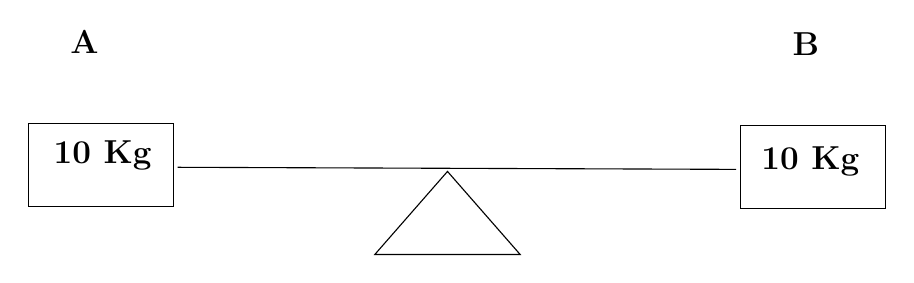
\begin{tikzpicture}[x=0.75pt,y=0.75pt,yscale=-1,xscale=1]
%uncomment if require: \path (0,300); %set diagram left start at 0, and has height of 300

%Shape: Rectangle [id:dp1922856828849877] 
\draw   (100,108) -- (170,108) -- (170,148) -- (100,148) -- cycle ;
%Shape: Rectangle [id:dp21830586730200763] 
\draw   (443,109) -- (513,109) -- (513,149) -- (443,149) -- cycle ;
%Straight Lines [id:da679579580856064] 
\draw    (172,129) -- (441,130) ;
%Shape: Triangle [id:dp34048765196571873] 
\draw   (302,131) -- (337,171) -- (267,171) -- cycle ;

% Text Node
\draw (111,115) node [anchor=north west][inner sep=0.75pt]  [font=\large] [align=left] {\textbf{10 Kg}};
% Text Node
\draw (452,118) node [anchor=north west][inner sep=0.75pt]  [font=\large] [align=left] {\textbf{10 Kg}};
% Text Node
\draw (119,62) node [anchor=north west][inner sep=0.75pt]   [align=left] {\textbf{{\large A}}};
% Text Node
\draw (467,63) node [anchor=north west][inner sep=0.75pt]   [align=left] {{\textbf{{\large B}}}};


\end{tikzpicture}

Baseado nesse conceito desenhe nas questões abaixo.


\begin{choice}

\choice  Desenhe a imagem quando {\bfseries A} for removido 5 kg.

\blank[blank-style={\phantom{#1}},width=20\linewidth]{}


\choice Desenhe a imagem quando {\bfseries A} for adicionado 10 kg.


\blank[blank-style={\phantom{#1}},width=5\linewidth]{}

\end{choice}
\end{exercise}


\collectexercisesstop{Adaptadas-Estequiometria}






\collectexercises{Adaptadas-Termoquimica}

\begin{multicols}{2}
\textbf{LEIA O TEXTO ABAIXO}

\textbf{Termoquímica:} É o estudo das quantidades de calor liberadas e absorvidas durante as transformações de estado físico, reações químicas etc\ldots{}

\textbf{Entalpia (H):} Entalpia é o conteúdo de calor de um sistema, à pressão constante. Não é possível medir a entalpia absoluta de um sistema por isso, mede-se a variação de entalpia (\(\Delta\)H) da reação

As reações e transformações quanto a entalpia são classificadas em \textbf{endotérmicas} e \textbf{exotérmicas}.

\section{Reações  Exotérmicas}
\label{sec:orgde52bce}
Nas reações exotérmicas, ocorre liberação de calor (o sistema esquenta), a entalpia dos produtos (\(\mathrm{H_P}\)) é menor do que a entalpia dos reagentes (\(\mathrm{H_R}\)) e o  \textbf{\(\Delta\)H=(–)}. De outra forma podemos concluir que a reação caminha de um estado de maior de energia a para um de menor energia, logo, o excesso é liberado.

Genericamente, temos:
Sendo a reação química representada de forma por: 
\begin{reactions*}
a A   +  b B   -> &  c C + d D \\
 (Reagentes)     & \; \;         (Produtos)
\end{reactions*}

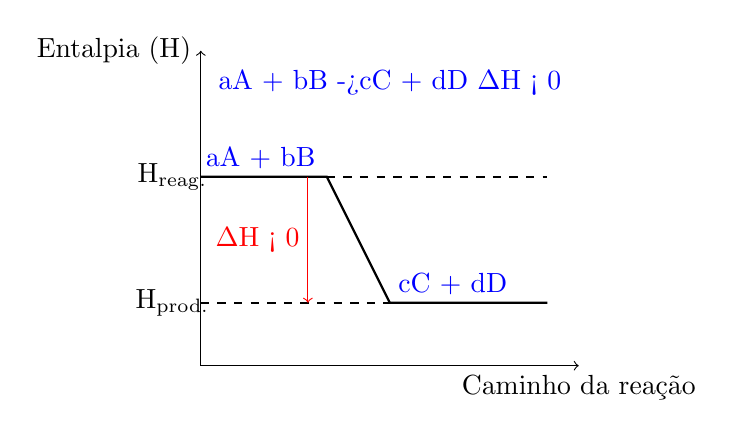
\begin{tikzpicture}[scale=.8]
		%% 
		% horizontal axis
		\draw[->] (0,0) -- (6,0) node[anchor=north] {Caminho da reação};
		% labels
		% vertical axis
		\draw[->] (0,0) -- (0,5) node[anchor=east] {Entalpia (H)};
		% nominal speed
		\draw[thick,dashed] (2,3) -- (5.5,3);
		\draw[thick,dashed] (0,1) -- (3,1);
		% Us
		%\draw[thick] (0,1) -- (2,1) -- (3,3)--(5.5,3);
		\draw (-.45,1) node {$\mathrm{H_{prod.}}$};
		\draw (-.45,3) node {$\mathrm{H_{reag.}}$};
		% Psis
		\draw[thick] (0,3) -- (2,3) -- (3,1)--(5.5,1);
		\draw[blue] (0.95,3.3) node {aA + bB}; %label
		\draw[blue] (4,1.3) node {cC + dD}; %label
		\draw[->,red] (1.7,3)--(1.7,1); 
		\draw[red](0.9,2) node {$\Delta$H < 0};
		\draw[blue](3,4.5) node {\ch{aA + bB ->cC + dD} $\Delta$H < 0};	
\end{tikzpicture}


\section{Reações  Endotérmicas}
\label{sec:orgaa0cbb7}
Nas reações endotérmicas, ocorre \textbf{absorção} de calor (o sistema \textbf{esfria}), a entalpia dos produtos (\(\mathrm{H_p}\)) é \textbf{maior} do que a entalpia dos reagentes (\(\mathrm{H_r}\)) e o  \textbf{\(\Delta\)H = ( + )}. De outra forma podemos concluir que a reação caminha de um estado de menor de energia a para um de maior energia, logo, a diferença que falta de energia é absorvido.

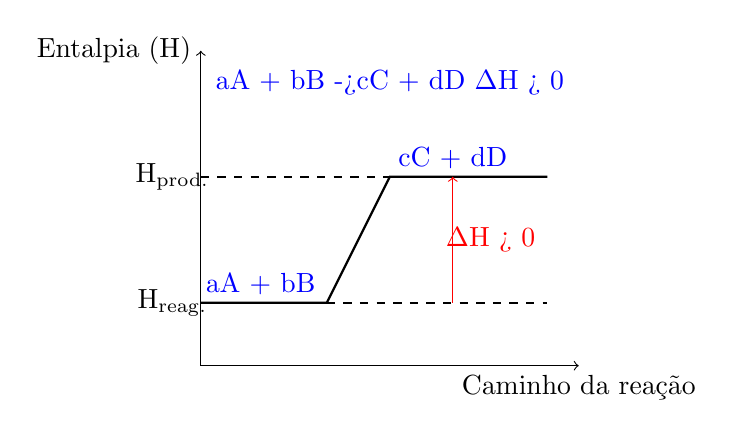
\begin{tikzpicture}[scale=.8]
	%% 
	% horizontal axis
	\draw[->] (0,0) -- (6,0) node[anchor=north] {Caminho da reação};
	% labels
	% vertical axis
	\draw[->] (0,0) -- (0,5) node[anchor=east] {Entalpia (H)};
	% nominal speed
	\draw[thick,dashed] (0,3) -- (3,3);
	\draw[thick,dashed] (2,1) -- (5.5,1);
	% Us
	\draw[thick] (0,1) -- (2,1) -- (3,3)--(5.5,3);
	\draw (-.45,1) node {$\mathrm{H_{reag.}}$};
	\draw (-.45,3) node {$\mathrm{H_{prod.}}$};
	% Psis
%	\draw[thick] (0,3) -- (2,3) -- (3,1)--(5.5,1);
	\draw[blue] (0.95,1.3) node {aA + bB}; %label
	\draw[blue] (4,3.3) node {cC + dD}; %label
	\draw[->,red] (4,1)--(4,3);
	\draw[red](4.6,2) node {$\Delta$H > 0};
	\draw[blue](3,4.5) node {\ch{aA + bB  ->cC + dD} $\Delta$H > 0};	
\end{tikzpicture}
\end{multicols}
\vspace{1cm}
{\bfseries Continua na próxima página}


\newpage
\section*{Questões}


\begin{exercise}
Observe a tirinha abaixo

\begin{figure}[ht]
\centering
\includegraphics[scale=0.3]{Adaptadas/fogo2.png}
\end{figure}

Considerando que a geladeira absorve calor qual seria o valor da entalpia ( $\Delta$H )

\begin{choice}(3)
\choice positivo
\choice negativo
\choice zero
\end{choice}
\end{exercise}

\begin{exercise}
Qual das imagens abaixo é uma reação \textbf{EXOTÉRMICA}

\begin{choice}(3)
\choice \includegraphics[scale=.4]{Adaptadas/gelo.png}
\choice \includegraphics[scale=.3]{Adaptadas/carvao.png}
\choice \includegraphics[scale=.5]{Adaptadas/fotosintesse.png}
\end{choice}
\end{exercise}



\begin{exercise}
Qual das imagens abaixo é uma reação \textbf{ENDOTÉRMICA}

\begin{choice}(3)
\choice \includegraphics[scale=.3]{Adaptadas/gas.png}
\choice \includegraphics[scale=.3]{Adaptadas/carvao.png}
\choice \includegraphics[scale=.5]{Adaptadas/fotosintesse.png}
\end{choice}
\end{exercise}




\collectexercisesstop{Adaptadas-Termoquimica}









\collectexercises{Adaptadas-Eletroquimica}


\begin{tikzpicture}[line join=round, line cap= round]
  % CELLS AND ELECTRODES
  \begin{scope}
    \draw[thick,fill=gray!50] (0.5,1) rectangle (1,5);    % Zn electrode
    \draw[thick,rounded corners] (0,4) |- (4,0) -- (4,4); % left cell
    \clip[rounded corners]       (0,4) |- (4,0) -- (4,4) -- cycle;
    \fill[gray,opacity=0.3]   (0,0)   rectangle (4,3);    % ZnSO4 solution
  \end{scope}
  \begin{scope}
    \draw[thick,fill=orange!50] (8,1) rectangle (8.5,5);  % Cu electrode
    \draw[thick,rounded corners] (5,4) |- (9,0) -- (9,4); % right cell
    \clip[rounded corners]       (5,4) |- (9,0) -- (9,4) -- cycle;
    \fill[blue, opacity=0.2]    (5,0) rectangle (9,3);    % CuSO4 solution
  \end{scope}
  % SALINE BRIDGE
  \draw[thick] (3,1)   --++ (0,2.5) arc (180:0:1.5) --++ (0,-2.5);
  \draw[thick] (3.5,1) --++ (0,2.5) arc (180:0:1)   --++ (0,-2.5);
  % WIRE AND VOLTMETER
  \draw[thick, rounded corners=0.5 cm] (0.75,5) |- (8.25,7) -- (8.25,5);
  \begin{scope}[shift={(4.5,7)}]
  \draw[thick,fill=white] (0,0) circle (0.5);
    \foreach\a in{30,60,...,150}
    {%
      \draw[blue,thin] (\a:0.35) -- (\a:0.45);
    }
  \fill[blue] (0,0) circle (1pt);
  \draw[blue,thick,-latex] (0,0) -- (60:0.4);
  \end{scope}
  % ELECTRONS
  \begin{scope}[shift={(1.5,6.25)}]
    \draw[red,thick,rounded corners=0.3 cm,->] (-0.5,-0.5) |- (0.5,0.5);
  \end{scope}
  % SIGNS
  \draw[red,thick] (-0.5,5.5) circle (0.25);
  \draw[red,thick] (9.5,5.5)  circle (0.25);
  \draw[red,thick] (-0.7,5.5) -- (-0.3,5.5);
  \draw[red,thick] (9.3,5.5)  -- (9.7,5.5);
  \draw[red,thick] (9.5,5.3)  -- (9.5,5.7);
  % LABELS
  \node at (4.5,8)    {Voltimetro};
  \node at (4.5,5.5)  {Ponte Salina  (\ch{KC$\ell$})};
  \node at (-0.5,5)   {Ânodo};
  \node at (-0.5,4.5) {(Oxidação)};
  \node at (9.5,5)    {Cátodo};
  \node at (9.5,4.5)  {(Redução)};
  \node[red] at (1.5,6.25) {\ch{e^-}};
  % CHEMISTRY
  \node at (2,-0.5) {\ch{ZnSO4}};
  \node at (7,-0.5) {\ch{CuSO4}};
  \node at (0.75,2) {\ch{Zn}};
  \node at (8.25,2) {\ch{Cu}};
  \node at (0.85,2) [right] {\small\ch{-> Zn^2+}};
  \node at (8.15,2) [left]  {\small\ch{Cu^2+ ->}};
\end{tikzpicture}


Observe a figura acime e responda as questões a seguir 

\begin{exercise}
Qual a  
\end{exercise}



\collectexercisesstop{Adaptadas-Eletroquimica}
\end{document}
